\documentclass[11pt]{article}

\usepackage[english]{babel}
\usepackage[utf8]{inputenc}
\usepackage{amsmath}
\usepackage{graphicx}
\usepackage[colorinlistoftodos]{todonotes}
\usepackage{booktabs}
\usepackage{dcolumn}
\usepackage{hyperref}
\usepackage[margin=1in]{geometry}
\hypersetup{
	colorlinks=true,
	linkcolor=blue,
	filecolor=magenta,      
	urlcolor=blue,
}

\begin{document}
\begin{center} 
\Large The Need for More Holistic Interventions and Long-Term Evaluations \\ 
in Gender \& Development \\ 
\vspace{6 pt}
\normalsize Marisa L. Henry\\
29 March 2019
\end{center} 

\linespread{1.25}
There is no question that educational gender parity is good for everyone. When women have equal access to quality education, they are empowered to have greater control over their futures. In addition to a number of social and health benefits, women who are more educated have higher earning potentials. This improves their own personal financial stability and contributes to societal economic development and \href{https://www.economist.com/finance-and-economics/2015/09/24/the-power-of-parity}{national gross domestic product}. 

Although women today are more educated than ever before, in most regions of the world they continue to lag men in total years of schooling (Figure \ref{fig:yrschratio}). For example, while women and men in Latin America and the Caribbean achieve roughly equal levels of education, in 2010 women aged 15 and over in South Asia had just 4.8 years of schooling on average compared to the average 7.3 years achieved by men. 

\begin{figure}[h!]
	\centering
	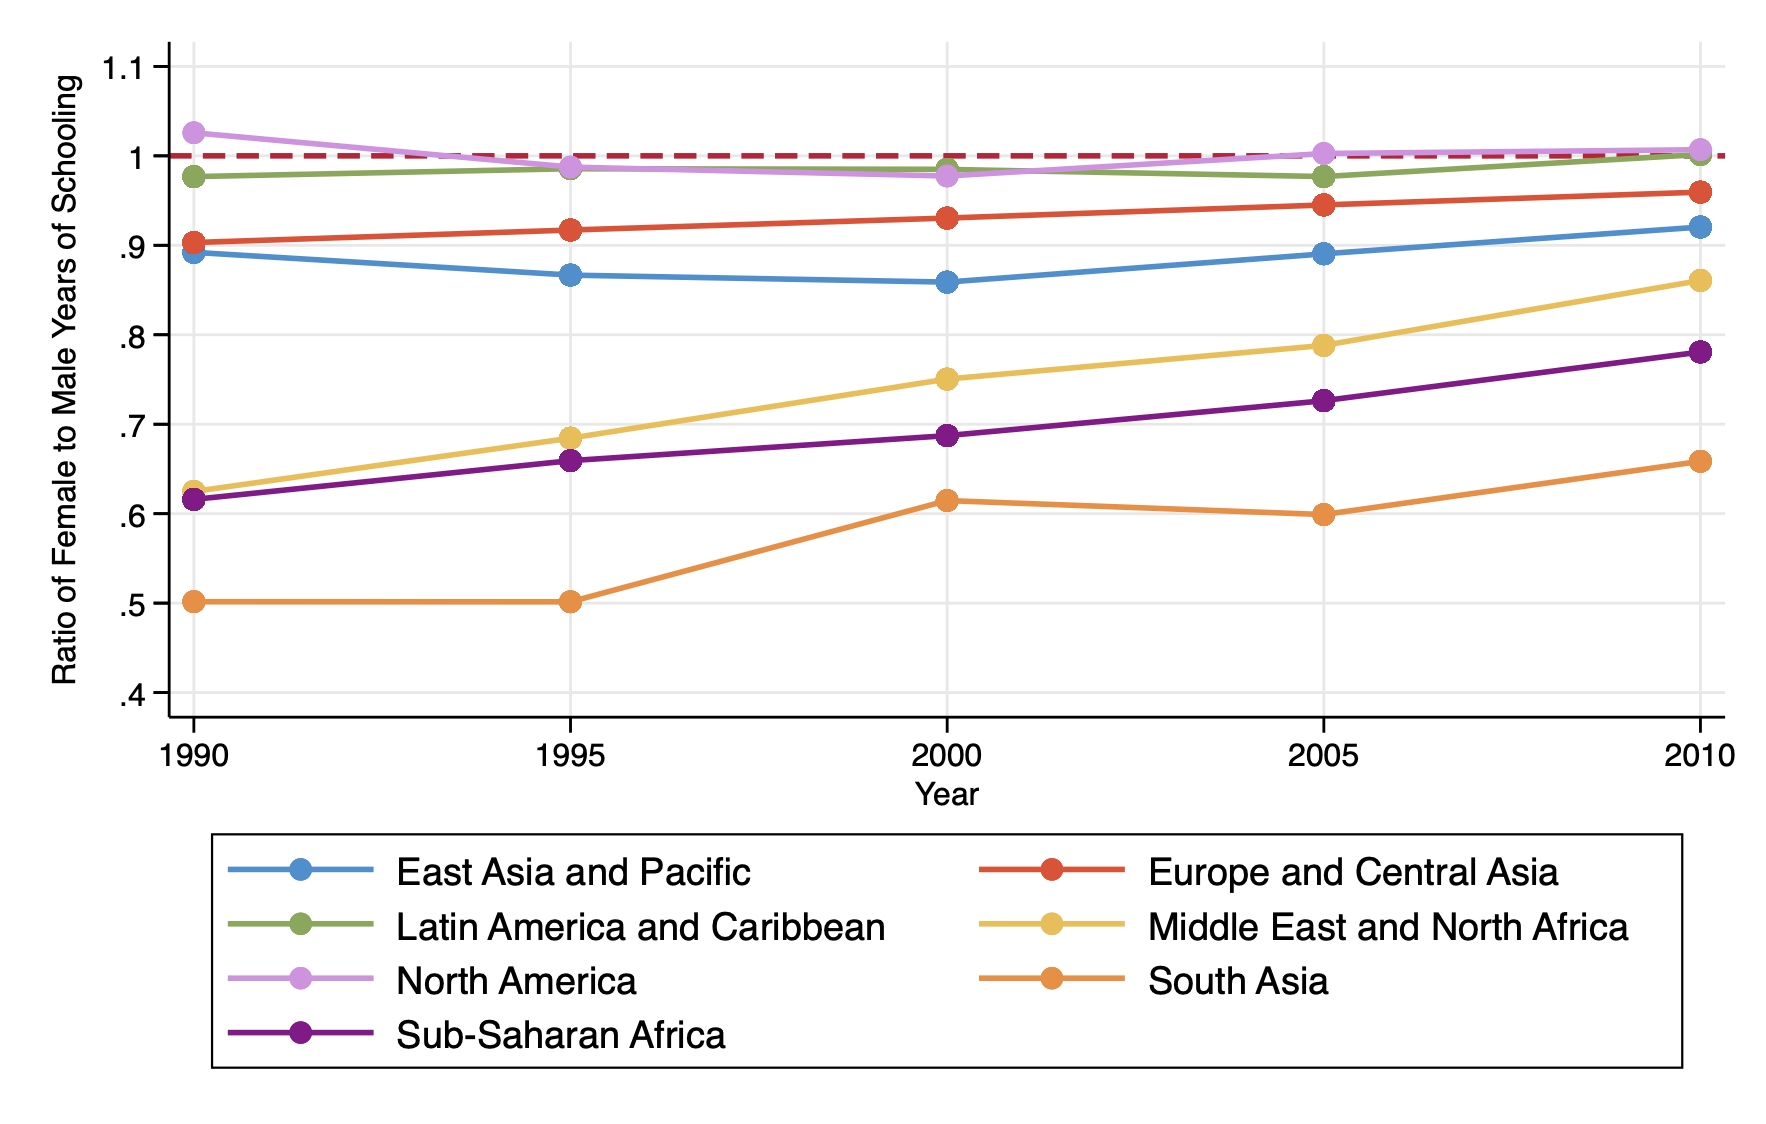
\includegraphics[width=0.9 \linewidth]{yrsch_ratio.png}
	\caption{\small Ratio of female to male years of schooling (population 15 years and over) by World Bank region, 1990 to 2010. A ratio of one indicates gender parity. Regional averages are calculated using country-level data from the \href{http://www.barrolee.com/}{Barro-Lee dataset}, weighted by country populations.}
	\label{fig:yrschratio}
\end{figure}

There also remains a global gender gap in labor force participation rates (LFPRs). In 2010, 49 percent of women (aged 15 and over) were part of the labor force, making up just \href{https://wol.iza.org/articles/female-labor-force-participation-in-developing-countries/long}{39 percent} of the total working population. Rates of participation also vary drastically by region: in 2010, the female LFPR was just 27 percent in the Middle East and North Africa compared to 60 percent in Sub-Saharan Africa. 

There is abundant evidence demonstrating we have made progress towards closing these gender gaps in education and the labor force. \href{https://data.unicef.org/topic/gender/gender-disparities-in-education/}{Data from UNESCO} shows most countries have achieved gender parity in primary school enrollment, and in North America, Latin America and the Caribbean women actually achieve more tertiary education than men. Over the last decade, development economists have conducted hundreds of experimental and quasi-experimental studies to quantify the effects of various interventions on educational outcomes and economic empowerment. In 2015, the UN endorsed a global goal of achieving gender equality by approving the
\href{https://sustainabledevelopment.un.org/}{Sustainable Development Goals (SDGs)} that include dozens of targets related to gender (see SDG 4 on education, SDG 5 on gender equality, and SDG 8 on economic growth and work). 

Looking only at these statistics and aspirational goals, however, ignores the challenges remaining in achieving gender equality in education and the labor force. Much of the current work in developing and evaluating interventions to improve education and economic empowerment takes a reductionist approach, focusing on specific points along the pathway from education to labor force participation and quantifying success based on short-term outcomes\footnote{Similar statements can be made about a range of social programs beyond just gender equality.}.To push gender equality forward, we need more holistic programs and long-term program evaluations of the right metrics. 

While ``targeted'' interventions that estimate short-term effects of specific programs advance research and provide valuable evidence for policy makers, they generally reveal little-to-nothing about the best combination of policies and programs to support women throughout their education and into the labor force. Even general poverty reduction efforts like cash transfers aren't enough to answer this important question. We can see some evidence of a gap between educational attainment and labor force participation by regressing the change in labor force participation rates on the change in female years of schooling over the same period. As shown in Figure \ref{fig:LFPRFyrsch} and Table \ref{tab1}, there is no association between the recent increases in female years of schooling and female labor force participation, even when adjusting for regional fixed effects. 

% If the ultimate goal is gender equality as expressed in the SDGs, we need better data on holistic gender empowerment programs. 

We also need more data on the long-term impacts of programs and policies. As noted in a recent \href{https://www.nber.org/papers/w25356}{working paper} of long-run impacts in development economics, we know little about long-term effects of development programs \footnote{This is an issue in evaluating social programs everywhere, not just in international development, as noted in  \href{texthttps://www.straighttalkonevidence.org/2019/04/03/beware-the-pitfalls-of-short-term-program-effects-they-often-fade/}{this post} from Straight Talk on Evidence.  \href{https://www.straighttalkonevidence.org/2019/04/30/not-all-program-effects-fade-new-report-on-the-project-quest-rct-shows-sizable-nine-year-earnings-gains-for-low-income-workers/}{Another post} from Straight Talk on Evidence highlights an exceptional example of a long-term RCT evaluation of a workforce training program for low-income individuals.}. However, the review also notes early studies in cash transfer programs that began in the 2000s may be amendable to long-term follow-ups. Additionally, they discuss methods to make the long-run program evaluations more successful, including alternative research design and data from utilizing administrative sources, remote sensing, and cell phones.

% Further, the little evidence that is available on long-term outcomes suggests that certain educational and conditional cash-transfer interventions have persistent effects. 

In addition to pursuing longer-term evaluations of experimental interventions, researchers should continue to conduct quasi-experimental studies that estimate causal effects using observational data. Methods like instrumental variables, difference-in-difference, regression discontinuity, and propensity score matching and weighting enable estimation of causal effects from programs and policies without randomization. While experimental studies are typically considered the ``gold standard'' for causal inference, the \href{https://onlinelibrary.wiley.com/doi/abs/10.1002/sim.2739}{careful design} of observational studies can enable exploration of a broader set of important causal questions, including long-term effects.

\begin{figure}
	\centering
	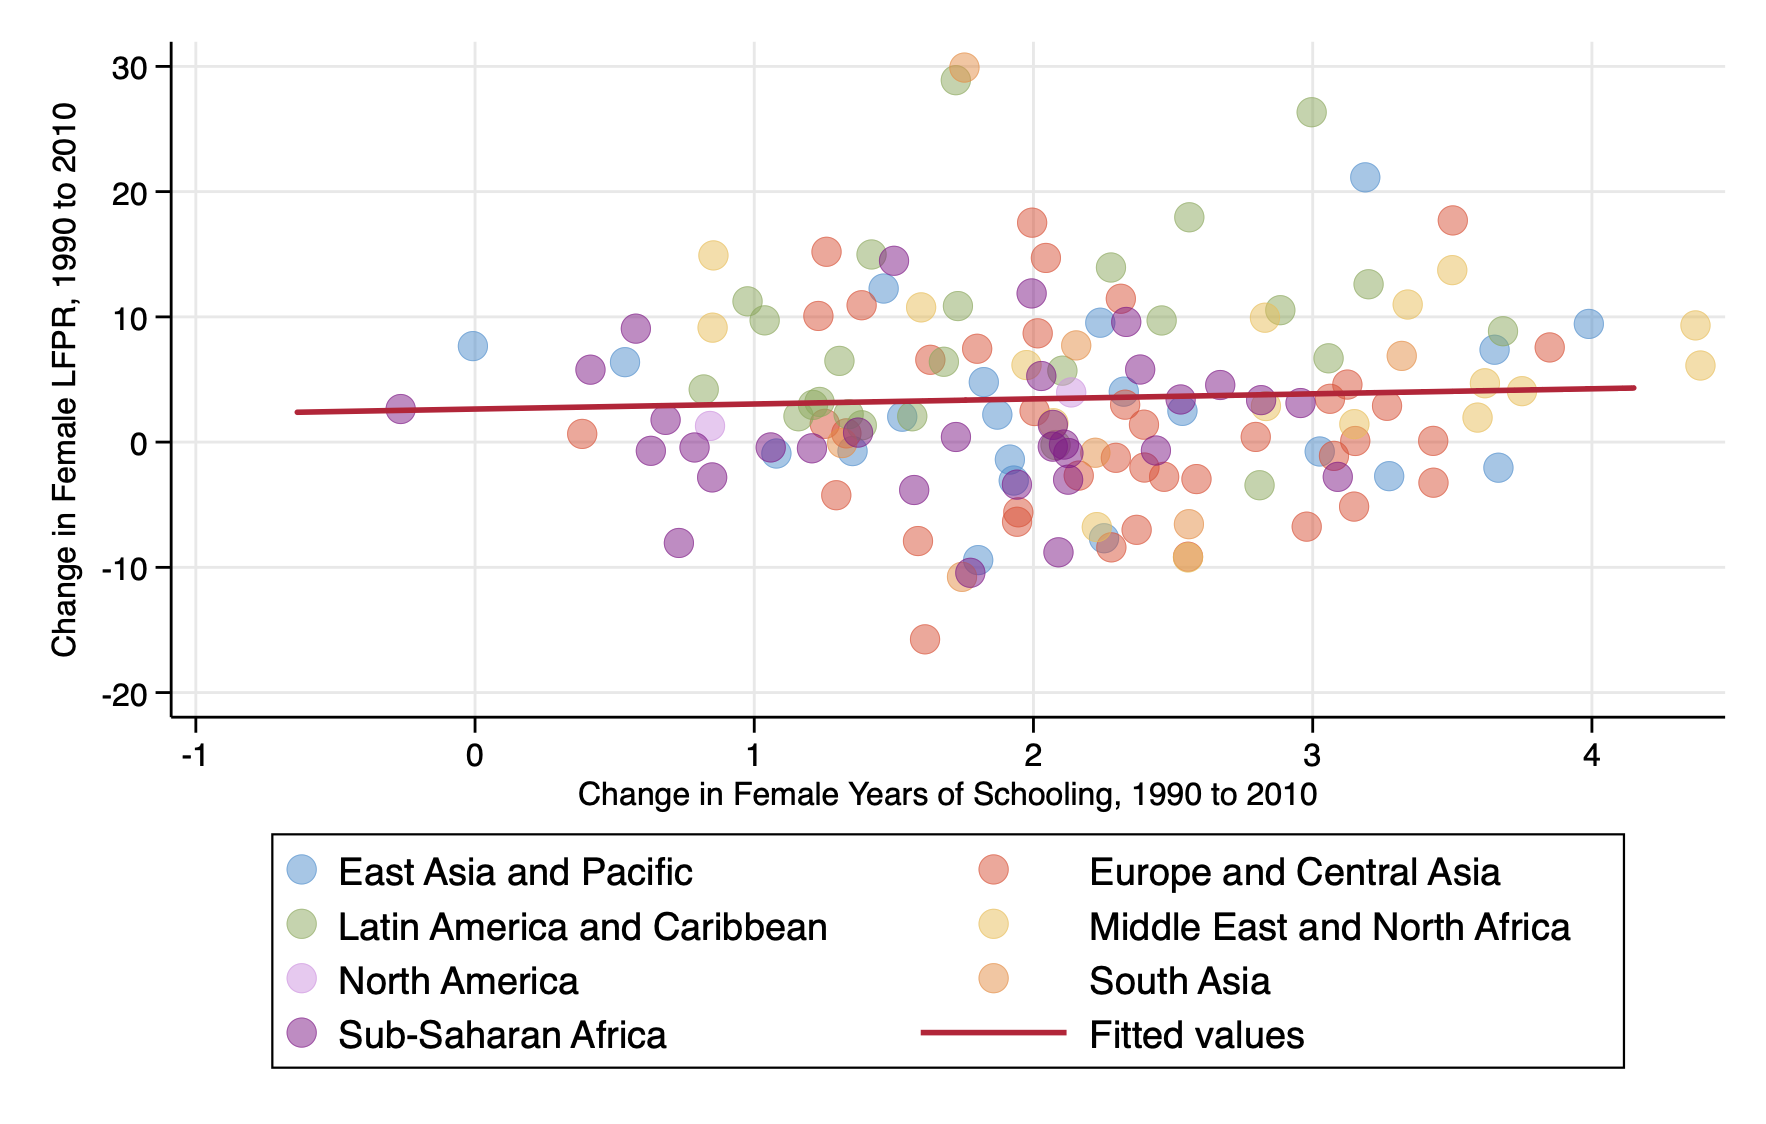
\includegraphics[width=0.9 \linewidth]{LFPRF_yrsch.png}
	\caption{\small Change in country-level female labor force participation rates vs the change in years of schooling (both population 15+), 1990 to 2010. Educational attainment data from the Barro-Lee dataset and labor force participation rates from the World Bank World Development Indicators database. }
	\label{fig:LFPRFyrsch}
\end{figure}

This call for more holistic programs and long-term evaluations isn't to say that we shouldn't continue to design and test focused, short-term programs. It may be that these more reductionist approaches actually achieve better long-term outcomes for women than comprehensive programs. Taking a more holistic approach to the design of future interventions will provide evidence of the best ways to shift the next generation through education and into empowering employment opportunities. 

% A World Bank survey (https://openknowledge.worldbank.org/bitstream/handle/10986/31327/WBL2019.pdf) of 187 economies, published last month, found that women had, on average, three-quarters of the legal and employment rights of men. The survey asked questions such as whether women were free to travel and open a business, if they had property rights and if they were protected from sexual harassment. In the Middle East and north Africa, women were found on this basis to have less than half the rights of men (Saudi Arabia was ranked lowest of all the countries surveyed). Only in six countries (Belgium, Denmark, France, Latvia, Luxembourg and Sweden) did the law and society grant women equal rights. https://www.economist.com/business/2019/03/09/a-small-step-for-women 
% Interventions that estimate effects on educational and employment outcomes include both ``targeted'' interventions (e.g. the impact of educational materials or highly trained teachers) and general poverty reduction efforts (e.g. cash transfers). Both are important, but neither provides insight into programs to support women for a longer term, throughout schooling and the transition to formal employment. The design and evaluation of holistic gender empowerment programs could help fill this gap.
% For example, \href{https://www.aeaweb.org/articles?id=10.1257/app.3.1.91}{one study} estimates the effect of improved sanitary materials on girls' school attendance over 1 year. Even if each of these programs are ``successful'', they may still fail to accomplish the long-term goals necessary for gender equality as expressed in the SDGs. Some evidence of this can be seen by comparing increases in female years of schooling and female labor force participation over the same period. There is no association between the recent increases in female years of schooling and female labor force participation, even when adjusting for regional fixed effects (Figure \ref{fig:LFPRFyrsch}, Table \ref{tab1}). 
% Further, looking at labor force participation as a proxy for women's economic empowerment fails to distinguish between employment in informal and formal sectors. Research from the \href{https://www.ilo.org/global/publications/books/WCMS_626831/lang--en/index.htm}{International Labour Organization} found that in low- and middle-income countries, a higher proportion of women are in informal employment than men. These women typically get paid less and lack access to state social programs, like unemployment benefits and pensions, that are often designed only for formal employment. This results in lower financial stability with little to no social safety net to rely on.
% https://www.ilo.org/global/publications/books/WCMS_626831/lang--en/index.htm


\newpage


\begin{table}[htbp]\centering
\def\sym#1{\ifmmode^{#1}\else\(^{#1}\)\fi}
\caption{Regression of the change in female labor force participation from 1990 to 2010 against change in female years of schooling during the same period  \label{tab1}}
\begin{tabular*}{\hsize}{@{\hskip\tabcolsep\extracolsep\fill}l*{2}{c}}
\toprule
                    &\multicolumn{1}{c}{(1)}         &\multicolumn{1}{c}{(2)}         \\
\midrule
Change in Female Years of Schooling, 1990 to 2010&       0.440         &       0.336         \\
                    &     (0.534)         &     (0.643)         \\
\addlinespace
East Asia and Pacific&                     &           0         \\
                    &                     &         (.)         \\
\addlinespace
Europe and Central Asia&                     &      -1.511         \\
                    &                     &     (0.450)         \\
\addlinespace
Latin America and Caribbean&                     &       5.800\sym{**} \\
                    &                     &     (0.009)         \\
\addlinespace
Middle East and North Africa&                     &       2.290         \\
                    &                     &     (0.353)         \\
\addlinespace
North America       &                     &     -0.0300         \\
                    &                     &     (0.996)         \\
\addlinespace
South Asia          &                     &       0.871         \\
                    &                     &     (0.788)         \\
\addlinespace
Sub-Saharan Africa  &                     &      -1.605         \\
                    &                     &     (0.447)         \\
\addlinespace
Constant            &       2.485         &       2.162         \\
                    &     (0.130)         &     (0.338)         \\
\midrule
Observations        &         144         &         144         \\
\bottomrule
\multicolumn{3}{l}{\footnotesize \textit{p}-values in parentheses}\\
\multicolumn{3}{l}{\footnotesize \sym{*} \(p<0.05\), \sym{**} \(p<0.01\), \sym{***} \(p<0.001\)}\\
\end{tabular*}
\end{table}

% \input{LFPR_MF_sch.tex}


\end{document}